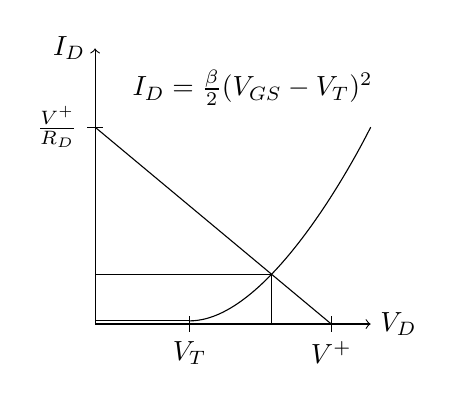
\begin{tikzpicture}
	\draw[->] (0,0) -- (0,3.5) node[left] {$I_D$};
	\draw[->] (0,0) -- (3.5,0) node[right] {$V_D$};
	\draw (0, 0.04) -- ++(1.2,0);
	\draw (1.2,0.04) .. controls (2.3,0.04) and (3.5,2.5) .. (3.5,2.5);
	\draw (2,3) node {$I_D = \frac{\beta}{2}(V_{GS} -V_T)^2$};
	\draw (1.2,0.1) -- +(0,-0.2) node[below] {$V_T$};
	\draw (0,0.63) -- ++(2.242,0) --  +(0,-0.63);
	\draw (0,2.5) -- (3,0);
	\draw (-0.1, 2.5) -- +(0.2,0);
	\draw (-0.1, 2.5) node[left] {$\frac{V^+}{R_D}$};
	\draw (3, 0.1) -- +(0, -0.2) node[below] {$V^+$};
\end{tikzpicture}